\documentclass[a4paper]{IEEEtran}

\usepackage[backend=bibtex]{biblatex}
\addbibresource{paper}
\usepackage{hyperref}
\usepackage{graphicx}

\title{Locating Data Flow Anomaly With Statistical Distance}
\author{Ruoyu Wang}
\date{2017.05.04}

\begin{document}
	\maketitle
	
	\begin{abstract}
		[abstract]
	\end{abstract}
	
	\section{Introduction}
		Big data industry has been blooming within this decade, reshaping the form of life and work across the globe. According to~\autocite{letouze2014official}, 1.2ZB data had been produced from 2012 to 2014. And the amount doubles every two years. Currently, there are totally 2.7ZB data in the digital universe~\autocite{bigDataStatistics}. Big data analysis has been widely adopted in scientific experiments~\autocite{nothaft2015rethinking}, electric business~\autocite{bronson2015open,sumbaly2013big,chen2016realtime}, healthcare~\autocite{groves2016big}, governments~\autocite{kim2014big} and many other fields.
		
		However, it will be harder in the future to harness the exploding volumes of data since problems have already appeared in data management and engineering, threatening trustworthiness and reliability of data flows inside working systems. Data error rate in enterprises is approximately 1\% to 5\%, and for some, even above 30\%~\autocite{saha2014data}.
		
		Those data anomalies may arise due to both internal and external reasons with respect to a certain system. From one hand, components inside the system may generate problematic source data. For example, in a sensor network, some sensors may generate erroneous data when it experiences power failure or other extreme conditions~\autocite{rassam2014adaptive}. Data packages will be lost if sensor nodes fail to connect to network or some sensor hub goes down~\autocite{herodotou2014scalable}. Also, human operators act as a heavily vulnerable part to bugs and mistakes. Some even deliberately modify system configurations for malicious compromises~\autocite{schuster2015vc3}. A study~\autocite{humanError} found that 65\% of organizations state that human errors are the main  cause of data problems.
		
		On the other hand, data manipulation~\autocite{dataManipulation} from outside hackers composes another potential threat of data quality and reliability. Taken Apache Hadoop as an example. It's security issues has long been discussed within communities and industry~\autocite{sharif2015current,terzi2015survey,jam2014survey,sharma2014securing}. As is shown in Figure~\ref{fig:hadoop-security}, the two basic vulnerabilities: \textit{lack of access control} and the \textit{absence of encryption} expose the entire cluster to dangerous threats. Data flows can be intercepted and modified; services can also be altered and blocked~\autocite{huang2014denial}. Although there are several frameworks(e.g. Kerberos, Sentry, Knox etc.) and algorithms providing basic protection~\autocite{zheng2017towards,sikdar2017spatio,xu2016high,yu2015enhancing,cohen2014towards}, clever attackers can always bypass the barriers and sneak into the core of data pipelines. Several approaches are developed as sentinels to detect probable infiltrations. However, these approaches are not able to locate corrupted data under carefully planned manipulations. Nor can they figure out the exact reasons and recover the original records. To locate and diagnose anomalies in data pipelines under carefully planned and disguised data manipulations are still on demand by industry and academia.
		
		\begin{figure}[!t]
			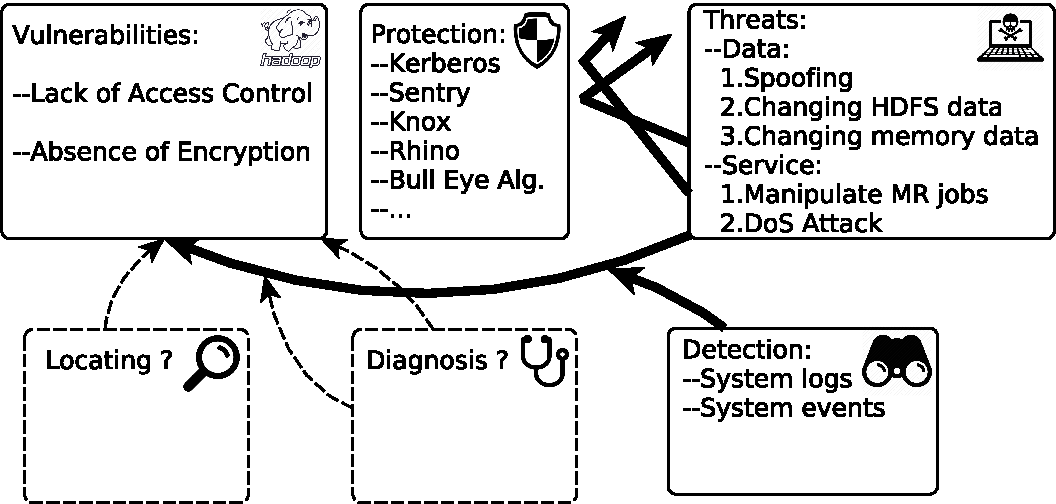
\includegraphics[width=\linewidth]{fig/HadoopSecurity}
			\caption{Security Issues of Hadoop Clusters}
			\label{fig:hadoop-security}
		\end{figure}

		\begin{figure}[!t]
			\centering
			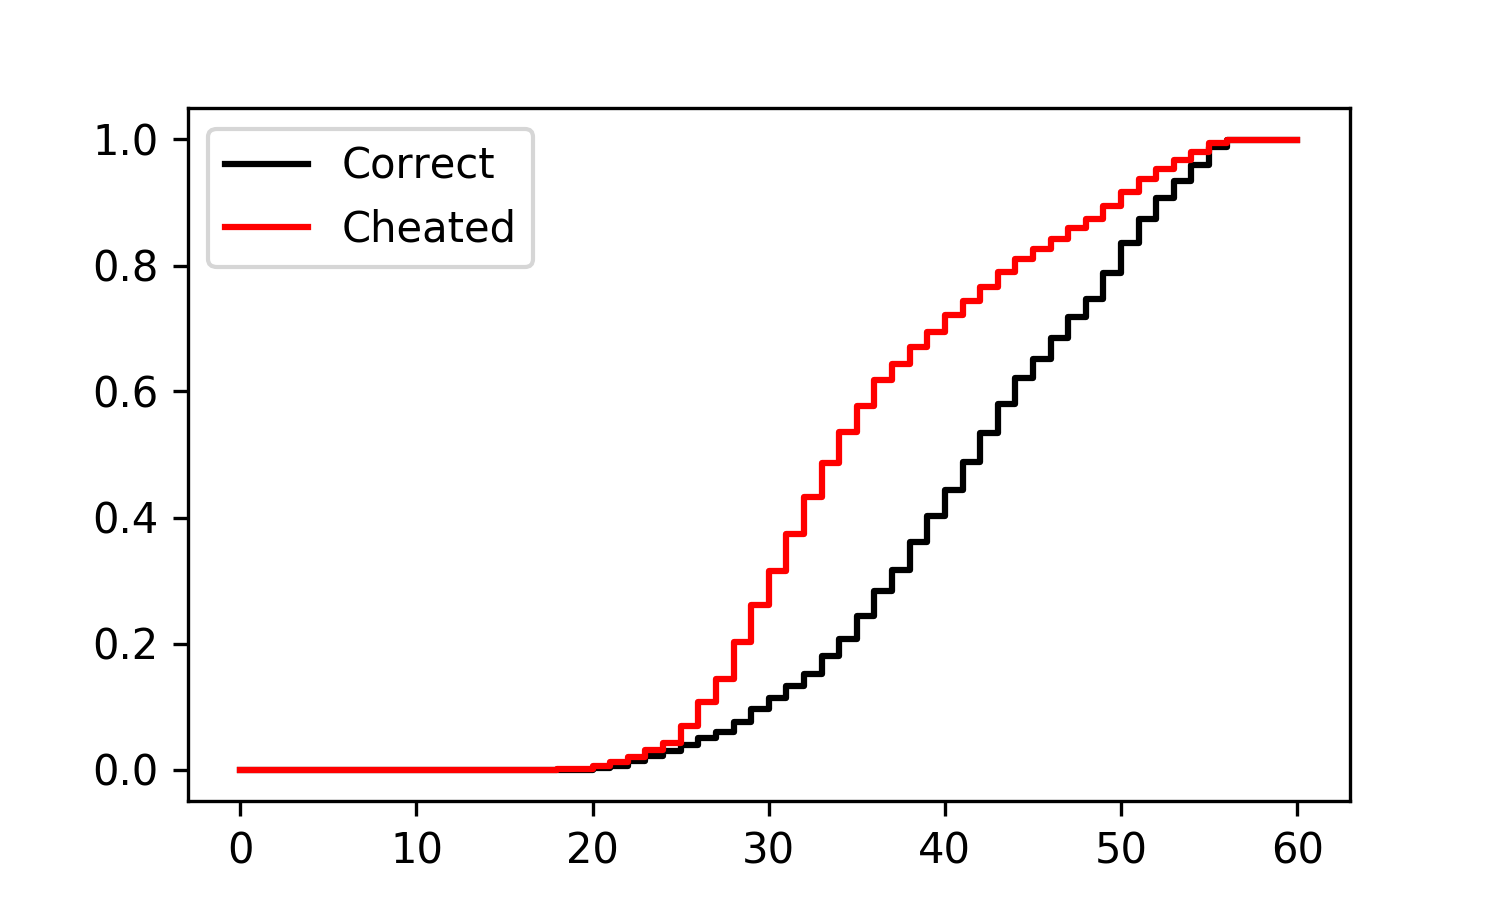
\includegraphics[width=\linewidth]{fig/ExampleEcdf.png}
			\caption{Example Cumulative Distribution Function of Original And Modified Data}
			\label{fig:example-ecdf}
		\end{figure}
		
		According to our observation, typical data manipulations on numerical data will lead to the drift of its distribution. For example, a Taobao online seller's transaction records can be ``click farmed'' to increase the volume of sales. Fig.~\ref{fig:example-ecdf} shows the sales distribution within one day. The curve for cheated data is emulated according to a popular method for click farming. It can be observed that there exists clearly a gap between these two distributions. 		
		%For example, in a sampled data set from Melbourne city pedestrian volume along main streets\footnote{https://data.melbourne.vic.gov.au/Transport-Movement/Pedestrian-volume-updated-monthly-/b2ak-trbp}, 20\% records were randomly selected and modified, the value set as a tenth of the original. The empirical cumulative distribution function of the two data sets are shown in Fig.~\ref{fig:example}, where there is clearly a gap between these distributions.
		These anomalies inside data pipelines will severely affect mining and learning algorithms and further change the final decision given by the entire system.
		
		In order to address issues resulted from data manipulation and pipeline errors, we propose a novel mechanism to detect and locate corrupted data within a data pipeline via statistical distance. As far as we know, this algorithm is the first attempt against data anomaly via statistical distance. Evaluations are performed on synthetic and real-world data sets, demonstrating the correctness and effectiveness of the mechanism.
		
		The rest of the paper is organised as follow: Section~\ref{sec:related-work} introduces recent works on data anomaly detection and pipeline error detection. Some background knowledge is provided in section~\ref{sec:preliminaries}. Then in section~\ref{sec:algorithm-details}, details of the detection and locating algorithm is proposed. Section~\ref{sec:evaluation} presents evaluation results and further findings of the algorithm. And all contents are concluded in section~\ref{sec:conclusion}.
	
	\section{Related Work}\label{sec:related-work}
		\subsection{Data Anomaly Detection}
			Anomaly detection, also known as outlier detection, has been studied for a long time and discussed in diverse research domains, such as fraud detection, intrusion detection, system monitoring, fault detection and event detection in sensor networks. According to a systematic classification in~\cite{chandola2009anomaly}, anomaly detection algorithms deal with input data in the form of points(or records), sequences, graphs and spatial relationships, where point data is the simplest and well studied, others are attracting more attention in new studies.
			
			Prevalent anomalies can be classified into \textit{Point Anomalies}, \textit{Contextual(or Conditional) Anomalies} and \textit{Collective Anomalies}. Point anomalies refers to an individual data instance that is considered anomalous with respect to others. But if it is anomalous only in certain circumstances or a specific context, the data is regarded as contextual anomaly. If a group of related data(e.g. a segment of sequence) instances is anomalous with respect to other groups in the data set(e.g. the entire sequence), it is called a collective anomaly.
			
			Detection approaches can be categorized into three types according to whether data is labeled: \textit{Supervised}, \textit{Semi-Supervised} and \textit{Unsupervised} anomaly detection. As the name suggests, supervised detection methods train models on completely labeled data while unsupervised detection leverages data without any labeling. Semi-supervised detection approaches train model on data that has labeled instances for only the normal class. Supervised detection is commonly applied when both normal and anomalous data can be obtained. When it comes to the circumstances that anomalous data is hard to obtain or there exist too many diverse types of anomalies to enumerate, semi-supervised or unsupervised approaches are usually taken into consideration.
			
			To make the final decision, detection algorithms mostly yield a score from each input instance, denoting how likely it is anomalous. The algorithm then selects top few as anomalies or compare the score with a threshold. Or, detection algorithms output a label on each instance, then decide whether each label belongs to the normal class.
			
			Currently, distance based~\cite{cao2014scalable,cao2017multi} and feature evolving algorithms~\cite{masud2013classification,li2015discovery,shao2014prototype} algorithms seize most attention. Others adopted tree isolation~\cite{zhang2017lshiforest}, model based~\cite{yin2016model} and statistical methods~\cite{zhu2002statstream} in certain applications.
			
			(or group anomaly)\cite{yu2015glad}.
		
		\subsection{Pipeline Error Detection}
		
		\subsection{Provenance}
		
		\subsection{Click Farming Detection}
	
	\section{Preliminaries}\label{sec:preliminaries}
		\subsection{Statistical Distance}
		
		\subsection{TDA?}
	
	\section{Algorithm Details}\label{sec:algorithm-details}
		\subsection{Technical Points}
			\textbf{[Can be divided and settled inside later two subsections]}
			\begin{enumerate}
				\item Which classifier should be chosen?
				\item How to determine the classifier threshold?\textbf{[fixed value, 3$\sigma$]}
				\item How to locate the compromised component?
				\item How to deal with slightly drifting distribution?
				\item .[to be continued \dots]
			\end{enumerate}
			
		\subsection{Basic Algorithm}
		
		\subsection{Dynamic Algorithm}
	
	\section{Evaluation}\label{sec:evaluation}
		\subsection{Experiment Environment}
		
		\subsection{Methodology}
			\textbf{Raise and answer some research questions. Present test background and methods.}
			
		\subsection{Experiment on Synthetic Data}
			\textbf{Test basic properties of statistical distance and algorithm}
		
		\subsection{Experiment on Real World Data}
			\textbf{Test performance of algorithm}
	
	\section{Conclusion}\label{sec:conclusion}
	
	\section*{Acknowledgement}
		
	\printbibliography
\end{document}




